\subsection{Misperception Transducer Trained Using EEG}
\label{ssec:eeg}

\newcommand{\specialcell}[2][c]{%
  \begin{tabular}[#1]{@{}c@{}}#2\end{tabular}}

Epoched and feature-coded EEG data {\em for the English syllables only}
were used to train a support vector machine classifier for each distinctive feature.
The classifiers were then used (without re-training) to classify the
EEG responses to the Dutch and Hindi syllables.
Fig.~\ref{fig:eeg_svm_eers} shows equal error rates of these
classifiers when applied to the three languages.

\begin{figure}
  \centerline{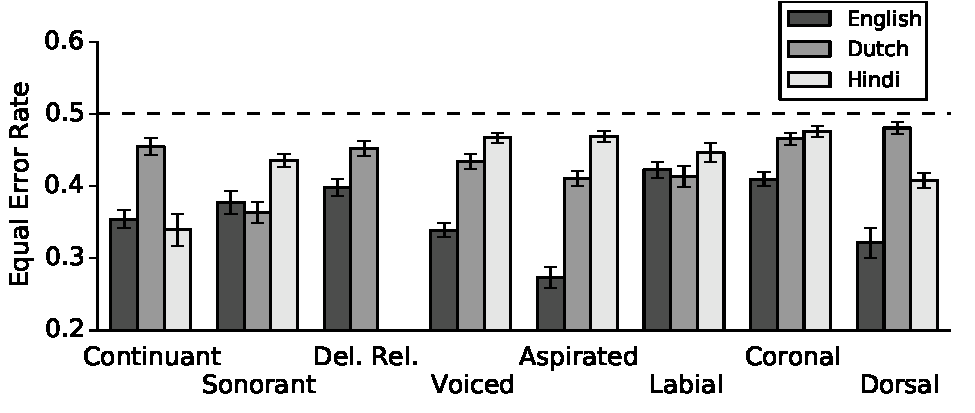
\includegraphics{../figs/eer-barplot/eer-barplot.pdf}}
  \vspace*{-0.3cm}
  \caption{Classifiers were trained to observe EEG signals, and to
    classify the distinctive features of the phone being heard.  Equal
    error rates are shown for English (the language used in training;
    train and test data did not overlap), Dutch, and Hindi.  Dashed
    line shows chance=50\%.}
  \label{fig:eeg_svm_eers}
\end{figure}

Eq.~(\ref{eq:dfdist}) defines a log-linear model of $\rho(\psi|\phi)$,
the probability that a non-English phoneme $\phi$ will be perceived as
English phoneme $\psi$.  Denote by $\rho_U(\psi|\phi)$ the model of
Eq.~(\ref{eq:dfdist}) with uniform weights for all distinctive
features. Denote by
$\rho_{EEG}(\psi|\phi)$ the same model, but with weights $w_k$ derived
from EEG measurements (Eq.~(\ref{eq:eegdist})).
Fig.~\ref{fig:eeg_confusions} shows these two confusion matrices:
$\rho_U(\psi|\phi)$ on the left, $\rho_{EEG}(\psi|\phi)$ on the
right. The entropy of the uniform weighting, $\rho_U(\psi|\phi)$, is
too low: when a Dutch phoneme $\phi$ has a nearest-neighbor
$\psi^*(\phi)$ in English, then few other phonemes are considered to
be possible confusions.  $\rho_{EEG}(\psi|\phi)$ has a very different
problem: since distinctive feature classfiers have been trained for
only a small set of distinctive features, there are large groups of
phonemes whose confusion probabilities can not be distinguished
(giving the figure its block-matrix structure).  The faults of both
models can be ameliorated by averaging them in some way, e.g., by
computing the linear interpolation
$\rho_I(\psi|\phi)=\alpha\rho_U(\psi|\phi)+(1-\alpha)\rho_{EEG}(\psi|\phi)$ for
some constant $0\le\alpha\le 1$.

\begin{figure}
  \centerline{
    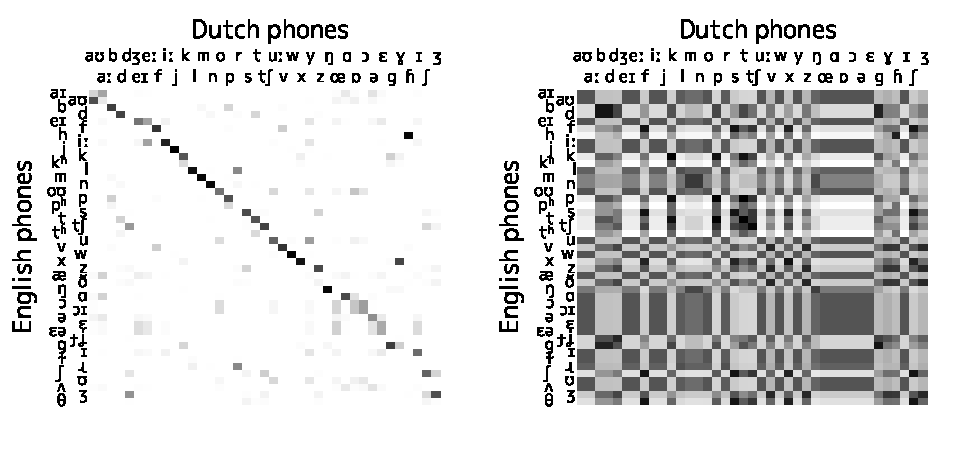
\includegraphics{../figs/confusion-matrix/confusion-matrices.pdf}
  }
    \vspace*{-0.3cm}
  \caption{Phone confusion probabilities between English and Dutch
    phones using models in which the log
    probability is proportional to distance between the corresponding
    distinctive features.  Left: all features have the same
    weight.  Right: feature weights equal negative log error rate of
    EEG signal classifiers.}
  \label{fig:eeg_confusions}
\end{figure}

In order to evaluate the effectiveness of the EEG-induced misperception 
transducer we looked at the label phone error rate of mismatched crowdsourcing
for the Dutch language when performed using 1)~a multilingual misperception
model $\rho(\lambda|\phi)$,
2)~feature-based misperception transducer computed using uniform 
weighting, $\rho_U(\psi|\phi)$, or 3) EEG-induced transducer combined with 
the feature-based transducer, $\rho_I(\psi|\phi)$. To combine the two 
transducers, the value of the parameter $\alpha$ was optimized on a 
separate development data set. As shown in Table~\ref{tbl:eegresults}, 
phone error rates were improved $1.5\%$ and $2.5\%$ relative to 
mismatched crowdsourcing by using the feature-based and combined 
misperception transducers (respectively). 

\begin{table*}
\begin{center}
\begin{tabular}{|c|c|c|c|}
  \hline
  & \specialcell{multilingual} & feature-based & \specialcell{EEG-induced\\+feature-based} \\
\hline
LPER & 70.43 & 69.44 & 68.61 \\
\hline
\end{tabular}
\vspace*{1mm}
\caption{\label{tbl:eegresults} Comparison of LPERs for probabilistic transcription of the Dutch evaluation set using different schemes to compute misperception G2Ps.}
\end{center}
\end{table*}


